\documentclass{article} 
% \usepackage[vietnamese]{babel}
\usepackage[utf8]{vietnam}
\usepackage{graphicx}
\usepackage{biblatex}
\bibliography{references.bib}

\graphicspath{{images/}}


\title{Báo Cáo về Mô Hình CARTE: Tiền Huấn Luyện và Chuyển Giao với Việc Học trên Dữ Liệu Bảng}
\author{Nguyễn Hữu Lộc - 23C15031 \and Lê Trường Vũ - 23C15042}
\date{09/02/2025}

\pagenumbering{arabic}

\begin{document}

\maketitle

\tableofcontents


\section{Giới thiệu sơ lược}
Các mô hình học máy tiền huấn luyện (pre-trained model) hiện nay đã trở nên phổ biến hơn nhiều và góp phần đáng kể vào sự phát triển của lĩnh vực trí tuệ nhân tạo trên nhiều loại dữ liệu khác nhau cả về mặt học thuật lẫn thương mại, nhất là trong các mảng về hình ảnh hay văn bản. Những mô hình này có thể được tải xuống từ các kho lưu trữ như HuggingFace, mang theo một lượng lớn thông tin ngầm và các phép biến đổi phức tạp, giúp tận dụng sức mạnh của học sâu ngay cả khi dữ liệu huấn luyện có quy mô nhỏ. Chính nhờ cách tiếp cận này, các mô hình nền tảng (foundation model), đặc biệt là các mô hình ngôn ngữ lớn (LLM), đã bùng nổ và định hình lại nhiều lĩnh vực.

Tuy nhiên, đối với dữ liệu dạng bảng thì dù loại dữ liệu này có ý nghĩa quan trọng trong môi trường doanh nghiệp và tổ chức nhưng tới hiện tại vẫn chưa có một mô hình nào có thể tạo nền tảng như vậy và trở ngại chính đền từ việc tích hợp dữ liệu từ nhiều bảng khác nhau. Đôi khi, các bảng có thể không chứa bất kỳ thông tin liên quan nào với nhau, và khi có, việc kết nối chúng lại trở thành một bài toán phức tạp trong lĩnh vực nghiên cứu cơ sở dữ liệu. Những thách thức điển hình bao gồm việc tìm mối tương ứng giữa các cột (đối sánh sơ đồ - schema matching) hoặc xử lý các nguồn dữ liệu có cách đặt tên khác nhau cho cùng một đối tượng (đối sánh đối tượng - entity matching). Do sự khác biệt này, việc huấn luyện trước trên dữ liệu bảng vẫn chưa khả thi, khiến phương pháp học sâu chưa thực sự đáng cân nhắc so với các phương pháp khác dựa trên cây quyết định.

Trong nghiên cứu này, nhóm đã đề xuất kiến trúc học máy CARTE (Context-Aware Representation of Table Entries) có thể học từ nhiều bảng dữ liệu mà không cần phải đối sánh sơ đồ hay đối sánh chuỗi ký tự. Cách tiếp cận cốt lõi của nhóm nghiên cứu là biểu diễn bảng dưới dạng đồ thị, trong đó các cột và giá trị trong bảng được ánh xạ thành các vector nhúng. Mô hình này được huấn luyện trước trên một cơ sở tri thức quy mô lớn, giúp nó có khả năng học hỏi từ một lượng lớn các đối tượng và mối quan hệ. Từ đó, mô hình có thể được tinh chỉnh cho các tác vụ cụ thể, ví dụ như những trường hợp hạn chế về dữ liệu huấn luyện, học từ nhiều bảng cùng lúc hay giúp bổ sung thông tin từ các nguồn dữ liệu thiếu liên kết.Thực nghiệm cho thấy CARTE mang lại sự cải thiện đáng kể về hiệu suất, vượt trội hơn hẳn so với 42 phương pháp cơ sở (baseline), bao gồm cả các phương pháp dựa trên cây quyết định và các kỹ thuật trích xuất đặc trưng khác, và thâm chí có hiệu quả cao đối với các bảng chứa dữ liệu dạng chuỗi văn bản, vốn rất phổ biến trong thực tế nhưng lại ít được đề cập trong các bộ dữ liệu chuẩn dành cho học máy.


\section{Các Nghiên Cứu Liên Quan}
Dữ liệu bảng đóng vai trò quan trọng trong nhiều ứng dụng thực tế, do đó, đã có nhiều phương pháp học sâu được phát triển để xử lý loại dữ liệu này. Tuy nhiên, trong hầu hết các trường hợp, các phương pháp này vẫn chưa thể vượt qua được những mô hình dựa trên cây quyết định. Mặc dù một số nghiên cứu đã chỉ ra rằng mạng nơ-ron có thể hoạt động tốt trên một số loại bảng nhất định, và nhiều kiến trúc hứa hẹn vẫn liên tục được nghiên cứu, nhưng để thực sự tạo vượt qua được thì các mô hình học sâu trên dữ liệu bảng cần phải tạo được một bước ngoặc lớn, chẳng hạn như khả năng tận dụng tri thức nền tảng tương tự như các mô hình ngôn ngữ lớn (LLM) đã làm.

Học chuyển giao trong dữ liệu bảng chủ yếu tập trung vào các trường hợp mà tập dữ liệu đích có cùng cấu trúc cột với tập dữ liệu nguồn. Một số phương pháp tiếp cận đã được đề xuất mô hình được huấn luyện trước trên một lượng dữ liệu dạng bảng lớn hơn nhưng không gán nhãn, hoặc sử dụng các bộ dữ liệu liên quan để thu hẹp khoảng cách giữa học sâu và mô hình cây quyết định, đặc biệt là trong bối cảnh dữ liệu y tế. 

Một số phương pháp có thể xử lý các bảng với cột khác nhau bằng cách ánh xạ dữ liệu sang không gian đặc trưng chung, điển hình là XTab, nhưng vẫn chưa đạt hiệu suất tốt hơn so với các mô hình cây hiện đại. Ngoài ra, cũng có các nghiên cứu hướng đến việc biểu diễn từng dòng dữ liệu dưới dạng vector nhúng để học trên nhiều bảng, đặc trưng có Transtab đã vượt qua một số mô hình cơ sở như là XGBoost. Tuy nhiên những phương pháp này có thể mở rộng cho nhiều ứng dụng khác nhau hay không.

Một số tiến bộ đã đạt được trong việc tiền huấn luyện mô hình trên dữ liệu bảng, chẳng hạn như TabPFN – một mô hình Transformer được huấn luyện trên dữ liệu tổng hợp, giúp cải thiện hiệu suất trên các tập dữ liệu nhỏ. Tuy nhiên, nó chưa có cơ chế xử lý tốt các cột dạng phân loại, vốn là một điểm mạnh của các mô hình cây. Các mô hình ngôn ngữ lớn (LLM) cũng đã được thử nghiệm cho dữ liệu bảng, chẳng hạn như TabLLM, trong đó dữ liệu bảng được chuyển thành những chuỗi token để ứng dụng vào việc tinh chỉnh các mô hình LLM. Tuy nhiên, do khó khăn trong việc xử lý số liệu trong các mô hình này, chúng vẫn chưa đủ tính cạnh tranh so với TabPFN hay cả những phương pháp dựa theo cây quyết định. 

Một thách thức quan trọng của dữ liệu bảng là sự xuất hiện của các giá trị rời rạc, thường được biểu diễn dưới dạng chuỗi văn bản. Một số nghiên cứu đã phát triển cách tiếp cận dựa trên biểu diễn chuỗi để hỗ trợ việc học từ loại dữ liệu này. Chẳng hạn, một số kỹ thuật biến đổi các cột khác nhau thành dạng số phù hợp cho việc học máy, hoặc sử dụng phương pháp nhúng trong đồ thị tri thức để mã hóa thông tin từ nguồn như Wikipedia. Tuy nhiên, những phương pháp này thường yêu cầu ánh xạ chính xác từng giá trị của cột sang một thực thể cụ thể liên kết đến Wikipedia, tạo ra nhu cầu phải xử lý thêm tác vụ đối sánh đối tượng (entity matching). 

Các mô hình thống kê truyền thống thường yêu cầu dữ liệu được tập hợp trong một bảng nhất quán, một bài toán thuộc lĩnh vực tích hợp dữ liệu. Một trong những thách thức quan trọng của lĩnh vực này là đối sánh sơ đồ (tìm cột tương ứng giữa các nguồn dữ liệu khác nhau) và đối sánh đối tượng (liên kết các chuỗi ký tự với đối tượng thực tế). Các phương pháp học sâu, đặc biệt là các mô hình dựa trên cơ chế tự chú ý, đã được áp dụng để hỗ trợ chuẩn hóa và tích hợp dữ liệu, giúp tự động hóa nhiều tác vụ mà trước đây cần đến sự can thiệp thủ công.

Tuy nhiên, nghiên cứu của nhóm nghiên cứu hướng đến một mục tiêu khác: thay vì dựa vào việc đối sánh rõ ràng các đối tượng hoặc sơ đồ, nhóm nghiên cứu tìm cách khai thác cấu trúc ngầm của dữ liệu để hỗ trợ các bài toán học máy mà không yêu cầu bất kỳ thao tác thủ công nào trong việc tìm kiếm nguồn dữ liệu liên quan. Đây là một vấn đề cấp thiết bởi hiện tại, có nhiều nhóm nghiên cứu đang nỗ lực xây dựng các kho dữ liệu bảng quy mô lớn nhưng do quy mô nhỏ của hầu hết các bảng dữ liệu hiện có và sự khác biệt lớn giữa các tập dữ liệu bảng. 

\section{Cách Mô Hình CARTE Học từ Dữ Liệu Bảng}
CARTE có thể học trên nhiều bảng dữ liệu khác nhau nhờ vào hai yếu tố chính: một cách biểu diễn mới cho đối tượng dạng bảng với cấu trúc đồ thị và một kiến trúc mạng nơ-ron sâu có khả năng nắm bắt ngữ cảnh(context) của bảng. Trong đó, cách biểu diễn đồ thị giúp đồng bộ hóa nhiều bảng dữ liệu vào cùng một không gian biểu diễn, làm cho việc tiền huấn luyện trên các dữ liệu nền tảng thiếu liên kết trước đây trở nên khả thi. Đồng thời, mạng nơ-ron sâu có khả năng nhận thức ngữ cảnh giúp truyền tải các thông tin nền sáng các tác vụ. 

\subsection{Biểu Diễn Đồ Thị của Đối Tượng Bảng}
Việc sử dụng đồ thị là yếu tố quan trọng để giúp khái quát hóa các đối tượng bảng (tabular entity). Một đồ thị $G$ bao gồm tập hợp các nút và cạnh, trong đó các nút biểu diễn đối tượng và các cạnh mô tả quan hệ giữa chúng. Đồ thị là công cụ mạnh mẽ để biểu diễn thông tin quan hệ giữa các đối tượng, và học sâu trên đồ thị đã được chứng minh là có tiềm năng lớn trong các tác vụ liên quan cơ sở dữ liệu có quan hệ (relational database).

CARTE tổ chức mỗi dòng dữ liệu trong bảng dưới dạng một đồ thị nhỏ. Giả sử bảng có $k$ cột, CARTE biểu diễn dòng dữ liệu thứ $i$ dưới dạng một đồ thị $G_i(X,E)$ trong đó $X$ và $E$ lần lượt là đặc trưng của nút và cạnh, được biểu diễn trong không gian $R^d$. Cấu trúc của $G_i(X,E)$ có dạng một đồ thị hình sao với $k-p_i$ nút lá, trong đó $p_i$ là số cột có giá trị bị thiếu trong dòng $i$. Trên mỗi đồ thị con này, các nút lá được gán nhãn theo giá trị ô dữ liệu và tên cột tương ứng.

Để biến đồ thị này thành đầu vào cho mạng nơ-ron, CARTE sử dụng một mô hình ngôn ngữ để khởi tạo các đặc trưng. Cụ thể là với các giá trị phân loại và tên cột, CARTE dùng mô hình ngôn ngữ để chuyển đổi giá trị thành dữ liệu dạng nhúng có $d$ chiều. Với các giá trị số, đặc trưng của nút được khởi tạo bằng cách nhân giá trị số với nhúng của tên cột tương ứng. Ví dụ, nếu một ô chứa giá trị 239 trong cột "H index", đặc trưng của nút đó sẽ là $239 \times E_{H index}$. Nút trung tâm của đồ thị được khởi tạo bằng giá trị trung bình của các nút lá và sẽ đóng vai trò là nút "readout". Trong mạng Neural Graph (Graph Neural Network - GNN), "node readout" (đọc nút) là một quá trình tổng hợp thông tin từ các nút (nodes) của đồ thị để tạo ra một biểu diễn đặc trưng có ý nghĩa cho toàn bộ đồ thị hoặc một phần của nó. 

\begin{figure} 
    \centering
    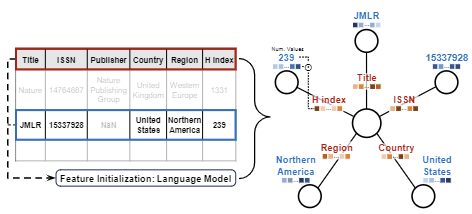
\includegraphics[scale = 1]{graphlet_representation_of_tabular_entity.png}
    \caption{CARTE biểu diễn mỗi hàng của bảng dưới dạng một đồ thị hình sao (graphlet). Các nút lá chứa giá trị ô và tên cột tương ứng. Các đặc trưng nút được khởi tạo bằng mô hình ngôn ngữ, trong đó giá trị số được điều chỉnh bằng đặc trưng cột. Nút trung tâm, ban đầu là trung bình của các nút lá, đóng vai trò tổng hợp thông tin của graphlet.}
    \label{fig:graphlet_representation_of_tabular_entity}
\end{figure}

Ưu điểm của cách biểu diễn đồ thị là cách tiếp cận này mang lại nhiều lợi ích. Giữ ngữ cảnh của dữ liệu bảng: Trong dữ liệu bảng, mỗi giá trị chỉ có ý nghĩa khi được xem xét trong ngữ cảnh của tên cột. Ví dụ như ở Hình \ref{fig:graphlet_representation_of_tabular_entity}, một dòng dữ liệu gồm các giá trị "JMLR", "15337928", "239" sẽ khó hiểu nếu không có tên cột đi kèm. Tuy nhiên, khi biết rằng chúng thuộc các cột "Title", "ISSN" và "H index", ta có thể nhận ra rằng đây là một tạp chí học thuật. CARTE khai thác ngữ cảnh này thông qua đồ thị, giúp mô hình học tốt hơn.

Vì các bảng có thể có số lượng cột khác nhau hoặc trật tự cột khác nhau, cách biểu diễn đồ thị của CARTE giúp kết nối dữ liệu mà không cần phải dữ liệu tên cột. Điều này mở ra khả năng học trên nhiều bảng mà không cần đối sánh sơ đồ. Bên cạnh đó, việc CARTE sử dụng mô hình ngôn ngữ để xử lý các giá trị dạng văn bản, danh mục và tên cột, giúp giảm bớt công đoạn tiền xử lý dữ liệu như mã hóa phân loại hay loại bỏ trùng lặp. Ngoài ra, CARTE có thể xử lý các từ vựng mở rộng, cho phép nhận diện những biến thể ngôn ngữ như “North America” và “Northern America” mà không cần ánh xạ thủ công.

Nhờ những đặc điểm trên, cách tiếp cận đồ thị của CARTE giúp khái quát hóa dữ liệu từ các bảng không đồng nhất, đưa tất cả các bảng vào cùng một miền biểu diễn mà không cần phải thực hiện đối sánh sơ đồ hay đối sánh đối tượng. Điều này tạo điều kiện cho việc học trên nhiều bảng, mở ra cơ hội tiền huấn luyện và học chuyển giao trên dữ liệu bảng một cách hiệu quả.


\subsection{Tiền Huấn Luyện Mô Hình từ Cơ Sở Tri Thức Lớn}
CARTE được tiền huấn luyện trên YAGO3 (Mahdisoltani et al., 2013), một cơ sở tri thức lớn được xây dựng từ Wikidata và các nguồn khác, chứa thông tin thực tế về thế giới. YAGO lưu trữ dữ liệu dưới dạng đồ thị tri thức, bao gồm các bộ ba (head, relation, tail). Ví dụ, bộ ba (“Louvre”, “is located in”, “Paris”) trong Hình 2 là một mẫu dữ liệu có thể tìm thấy trong YAGO. Phiên bản hiện tại của YAGO chứa hơn 18,1 triệu bộ ba với 6,3 triệu thực thể.

Trong phần này, chúng tôi mô tả quá trình tiền huấn luyện của CARTE, được tóm tắt trong Hình 2. Từ đồ thị tri thức, chúng tôi trích xuất các đồ thị con nhỏ hơn (graphlets) phù hợp để làm đầu vào cho CARTE. Để thực hiện học tự giám sát với hàm mất mát tương phản (contrastive loss), chúng tôi thêm vào batch các phiên bản bị cắt ngắn của các graphlets đã chọn. Thông qua quá trình huấn luyện, CARTE học cách tổng hợp thông tin dựa trên ngữ cảnh được cung cấp.

Graphlets cho tiền huấn luyện
Từ đồ thị tri thức lớn YAGO, chúng tôi xây dựng các graphlets nhỏ hơn có thể dùng làm đầu vào cho CARTE. Để tạo một graphlet phù hợp cho một thực thể, chúng tôi trích xuất tiểu đồ của nó trong phạm vi k quan hệ liên kết (k-hop relations). Để duy trì cấu trúc được trình bày trong Hình 1, đồng thời tận dụng thêm thông tin từ nhiều bước nhảy, chúng tôi đặt k=2, nhưng giới hạn số lượng quan hệ 1-hop và 2-hop lần lượt là 100 và 10.

Các graphlets từ bảng dữ liệu (Hình 1) sử dụng một token làm node trung tâm cho mỗi hàng, trong khi các graphlets từ đồ thị tri thức có thể sử dụng tên thực thể (ví dụ: “Louvre”). Để tránh sự khác biệt này, chúng tôi sử dụng một token làm node trung tâm, kèm theo một node bổ sung chứa tên thực thể và được kết nối bằng quan hệ “has name”. Cuối cùng, tương tự như Mục 3.1, chúng tôi khởi tạo các node và cạnh bằng cách sử dụng embedding từ mô hình ngôn ngữ FastText (Mikolov et al., 2017).

Tạo batch mẫu
Để tạo một batch mẫu với kích thước $N_b$, đầu tiên chúng tôi chọn các thực thể từ YAGO để đưa vào batch và tạo các graphlets tương ứng. Trong đó, 90\% $N_B$ được lấy từ các thực thể có ít nhất 6 quan hệ 1-hop, 10\% còn lại được lấy từ các thực thể khác. Lý do chính cho việc lấy mẫu như vậy là do phần lớn thực thể trong YAGO chỉ có một hoặc hai quan hệ 1-hop, trong khi dữ liệu dạng bảng thường có nhiều hơn (tương ứng với nhiều cột). Hơn nữa, giá trị 6 được chọn để đảm bảo rằng số quan hệ trung bình trong batch mẫu xấp xỉ 15.

Để áp dụng học tự giám sát với mất mát tương phản, chúng tôi tạo ra các mẫu dương bằng cách xóa một phần ngẫu nhiên (từ 30\% đến 70\%) số cạnh trong graphlets gốc. Hình 2 minh họa một graphlet của thực thể “Louvre” cùng với phiên bản bị cắt ngắn của nó.

Kiến trúc mô hình
Hình 3 mô tả kiến trúc của CARTE. Về cơ bản, CARTE sử dụng mô hình Transformer encoder truyền thống của Vaswani et al. (2017) và điều chỉnh nó thành một mạng đồ thị với cơ chế chú ý. Một thành phần quan trọng trong kiến trúc của CARTE là lớp tự chú ý (self-attention) tính toán mức độ quan trọng của các node và cạnh trong đồ thị. Trong mô hình đồ thị, cơ chế chú ý điều chỉnh tầm quan trọng của các node lân cận đối với một node nhất định.

Đối với dữ liệu bảng, điều này có nghĩa là xác định mức độ quan trọng của từng giá trị trong hàng, với ngữ cảnh được bổ sung bởi thông tin cột. Chúng tôi sẽ trình bày chi tiết về cơ chế chú ý của CARTE để nắm bắt ngữ cảnh và mối quan hệ giữa các thực thể.


\subsection{Tinh Chỉnh cho Tác Vụ}
Trong quá trình fine-tuning cho một tác vụ cụ thể, CARTE chỉ tái sử dụng một phần của kiến trúc đã được tiền huấn luyện (như trong Hình 3). Cụ thể, mô hình giữ lại:

Các lớp ban đầu xử lý node và cạnh (các khối màu xanh và đỏ).
Lớp “Aggregation \& Readout” tổng hợp thông tin từ các node và cạnh.
Không giống như nhiều phương pháp fine-tuning khác, cách tiếp cận này dựa vào đặc điểm của mạng nơ-ron đồ thị (GNN). Lý do là vì các bảng dữ liệu trong bài toán downstream (sử dụng mô hình để giải quyết bài toán cụ thể) có đồ thị đơn giản hơn so với trong giai đoạn tiền huấn luyện:

Đồ thị trong bài toán downstream có dạng ngôi sao (star-like structure, xem Hình 1), tức là một node trung tâm liên kết với các node còn lại.
Cấu trúc đồ thị của bảng downstream ít đa dạng hơn so với YAGO, tập dữ liệu gốc dùng để huấn luyện CARTE.
Số lượng biến rời rạc (cardinality) trong bảng downstream ít hơn, giúp mô hình dễ học hơn.
Nếu sử dụng một kiến trúc quá sâu, thông tin đặc trưng của các node có thể bị làm mờ dần qua các lớp (hiện tượng over-smoothing, Chen et al., 2020a; Rusch et al., 2023, được phân tích trong Phụ lục C.4). Vì vậy, CARTE áp dụng một nguyên tắc phổ biến trong mô hình đồ thị:

Số lớp chú ý (attention layers) được đặt bằng số bước quan hệ tối đa k-hop, với k = 1 trong trường hợp này.
Bộ phân loại cuối cùng chỉ đơn giản là một mạng nơ-ron tuyến tính.
Với mô hình cơ bản này, chúng tôi xem xét hai cách suy luận (inference) trên dữ liệu downstream:

\subsubsection{Suy luận trên dữ liệu bảng đơn}
Đây là trường hợp phổ biến nhất, trong đó chúng ta có một bảng dữ liệu duy nhất và cần dự đoán một biến mục tiêu (target variable). Trước khi biến đổi bảng thành đồ thị:

Biến số (numerical variables) được xử lý trước bằng phép biến đổi lũy thừa (power transform) (Yeo \& Johnson, 2000), giúp ổn định phân phối dữ liệu. Cách tiếp cận này đã chứng minh hiệu quả trong nhiều nghiên cứu trước đây (Hollmann et al., 2023; Cvetkov-Iliev et al., 2023).
Để tăng độ chính xác và tránh overfitting, chúng tôi sử dụng chiến lược bagging (Breiman, 1996):

\begin{itemize}
    \item Tạo nhiều mô hình bằng cách sử dụng các tập train-validation khác nhau.
    \item Dừng sớm (early stopping) dựa trên tập validation.
    \item Dự đoán cuối cùng là trung bình của các đầu ra từ các mô hình trên.
\end{itemize}

\subsubsection{Học chuyển giao từ một bảng nguồn sang bảng đích}
Chúng tôi cũng áp dụng CARTE cho học chuyển giao (transfer learning), khi có một bảng nguồn $X_S$có thể hỗ trợ dự đoán trên bảng đích $X_T$. Trong nhiều trường hợp, bảng nguồn có nhiều dữ liệu huấn luyện hơn bảng đích.

Quá trình fine-tuning trong học chuyển giao được thực hiện như sau:

Huấn luyện CARTE trên cả hai bảng nguồn và đích cùng lúc.

Do dữ liệu được biểu diễn dưới dạng đồ thị, việc fine-tuning có thể diễn ra mà không cần các cột giữa hai bảng phải khớp nhau.
Tuy nhiên, chúng tôi yêu cầu rằng nhãn đầu ra $y_X$ và $y_T$ của bảng nguồn và đích phải có mối quan hệ tương tự.
Điều chỉnh nhãn của bảng nguồn để phù hợp với bảng đích:

Nếu $y_T$ là biến phân loại: chuyển đổi $y_S$ từ bài toán hồi quy thành phân loại nhị phân.
Nếu $y_T$ là biến hồi quy: sử dụng nhãn phân loại nhị phân của bảng nguồn ({0,1}) và chuẩn hóa theo phương pháp standard scaling.
Lấy mẫu dữ liệu trong quá trình huấn luyện:

Với batch size 64, mỗi batch có 8 dòng từ bảng đích và phần còn lại từ bảng nguồn.
Dừng sớm (early stopping) dựa trên tập validation của bảng đích.
Tiếp tục sử dụng bagging, tức là xây dựng nhiều mô hình trên các tập validation khác nhau và lấy trung bình dự đoán.
Kiểm soát việc quá khớp với bảng nguồn:

Trong hầu hết các trường hợp, early stopping xảy ra trước khi tất cả dữ liệu của bảng nguồn được sử dụng.
Điều này giúp tránh overfitting vào bảng nguồn, do dữ liệu của bảng nguồn có thể không quan trọng bằng dữ liệu của bảng đích để dự đoán $y_T$ .
Kết hợp mô hình transfer learning với mô hình single-table:

Khi bảng nguồn không chứa đủ thông tin hữu ích, mô hình học chuyển giao có thể không tốt hơn so với mô hình chỉ sử dụng bảng đích.
Chúng tôi sử dụng softmax ensemble để kết hợp hai mô hình này. Trọng số của softmax được tính dựa trên điểm dự đoán từ tập validation, được chuẩn hóa bằng độ lệch chuẩn giữa các mô hình để điều chỉnh nhiệt độ (temperature scaling).

\subsubsection{Học chung trên nhiều bảng}
Trong bài toán học chuyển giao, việc chọn bảng nguồn phù hợp đóng vai trò quan trọng. Nếu có nhiều bảng dữ liệu thuộc cùng một lĩnh vực hoặc tổ chức, CARTE có thể khai thác tất cả các bảng này để tìm ra thông tin hữu ích nhất.

Giả sử có một bảng đích $X_T$ và tập hợp các bảng nguồn ${X_{S,1}, ..., X_{S,m}}$, chúng tôi tiến hành như sau:

Xây dựng từng mô hình học riêng lẻ:

Trước tiên, huấn luyện mô hình single-table trên $X_T$.
Sau đó, huấn luyện từng mô hình pairwise joint learner trên từng cặp ($X_T, X_{S,i}$).
Ensemble để chọn mô hình tốt nhất:

Không phải mọi cặp bảng đều mang lại thông tin hữu ích như nhau.
Chúng tôi sử dụng chiến lược ensemble như trên, kết hợp tất cả các mô hình học đôi (pairwise learners) và mô hình single-table.
Nếu tất cả các bảng nguồn đều hữu ích, chúng được kết hợp với trọng số bằng nhau.
Nếu một bảng nguồn cung cấp nhiều thông tin hơn hẳn, mô hình sẽ ưu tiên bảng đó trong quá trình dự đoán.



\section{Nghiên Cứu Thực Nghiệm}
\subsection{Cài Đặt Thực Nghiệm}

\subsection{Kết Quả trên Bảng Đơn}

\subsection{Học Đa Bảng}

\section{Bàn Luận và Kết Luận}

% \printbibliography

\end{document}